% Rahmen stecken, Business relationship is important for market analysis (example like VW) or stock price prediction. 2 features are presented which are useful as proxy for business relationship

The financial markets play a crucial role in global market economy. By supplying companies with capital they influence the economic development and thereby are partially responsible for the prosperity of today's society. Due to their promise of fast money and high returns, financial markets are a highly competitive field. This being said, stock prices not only reflect the value of a company's share but also temporal fluctuations caused by supply and demand among the investors. The Random Walk Theory, partly introduced by \citet{Regnault1863CalculBourse} and later disseminated by \citet{Malkiel1973AStreet}, hypothesizes that changes in stock prices follow a fair-game pattern, i.e. they are random and therefore not predictable. Since empirical findings led to the supposition that this theory does not explain the financial markets sufficiently, the influential theory of Efficient Market Hypothesis (EMH) by \citet{Bachelier1900TheorySpeculation} became popular over the last century, especially when it was formalized by \citet{Fama1965RandomPrices}. It states that each investor has access to all relevant information and acts rational. Based on these assumptions, the theory concludes that a stock price always reflects all available information. Hence, it should not be possible to outperform the market by picking undervalued stocks, i.e. exploiting arbitrage opportunities \cite{Franke2010StatisticsMarkets}. There are neither undervalued nor overvalued stocks. Nowadays, this hypothesis is still very popular but also treated with growing scepticism \cite{Hsu2016BridgingEconomists, KhadjehNassirtoussi2014TextReview, Yoo2005MachineEvaluation}. The huge amount of available information are difficult to grasp for investors and can be imprecise. Another theory taking this comprehended efficiency into account, is called Bounded Rationality \cite{Simon1955AChoice} and implies that stock prices not always reflect their real economical value \cite{Hsu2016BridgingEconomists}.
% Add Finding? Hsu et al.: weak form EMH: stocks can take some time to reflect all information
% \todo{Explain weak version of EMT more in detail?}
% Bounded Rationality: https://mpra.ub.uni-muenchen.de/83721/1/MPRA_paper_83721.pdf
% https://sci-hub.se/10.1007/978-3-319-66104-9


% Unfortunately, there are various external influences on the stock market which may violate empirical well-founded relations in the historical stock price data.

In order to cover a broad set of related information influencing stock prices, latest research considers unstructured information from newspapers and other media sources. To extract important data from the mainly textual data Natural Learning Processing (NLP) is necessary (e.g. \cite{Yoshihara2014PredictingNetworks}). One of the most important data sources are financial reports (e.g. so called SEC filings) which need to be filed by publicly traded companies with the United States federal Securities and Exchange Commission. For example, \citet{Lee2014OnPrediction} improved their baseline for predicting next day’s price movements by 10~\% (relative) using extracted features from financial reports.

A lot of related approaches try to incorporate events from the news since they might be helpful for comprehending and predicting the stock markets behaviour. However, the market does not only depend on those external influences. A lot of traded companies maintain business relationships with each other and thereby influence each others stock price. To give an example: if higher sales figures are to be expected for one company, investors might conclude the same for the suppliers of this company and the opposite for affected competitors. Reported news might only be consequences of those underlying relationships. Based on these assumptions, I hypothesize the business relations to have an impact on the stock prices.

%  
The remainder of this work is organized as follows: Section~\ref{section:problem_definition} gives a more specific problem definition of this work more. Subsequently, some background information about the financial markets and the later used statistical methods will be provided in Section~\ref{section:background}. In Section~\ref{section:methodology} the methods for feature extraction and hypothesis evaluation are outlined. In order to grasp the established methods for stock price modelling in combination with NLP, Section~\ref{section:related_work} presents related approaches. Section~\ref{section:data} introduces the two datasets for historical prices and financial news which will be used throughout the following sections. Preprocessing of stock prices from the American stock market and evaluation of their statistical properties will be conducted in Section~\ref{section:statistical_analysis}. Section~\ref{section:text_analysis} describes how business relationships are extracted from news articles based on occurrences of companies. Then, I will evaluate my hypothesis and discuss findings in Section~\ref{section:evaluation}. Finally, conclusions are drawn and an outlook of potential future work is provided in Section~\ref{section:conclusion}.





% \begin{figure}[h!]
%     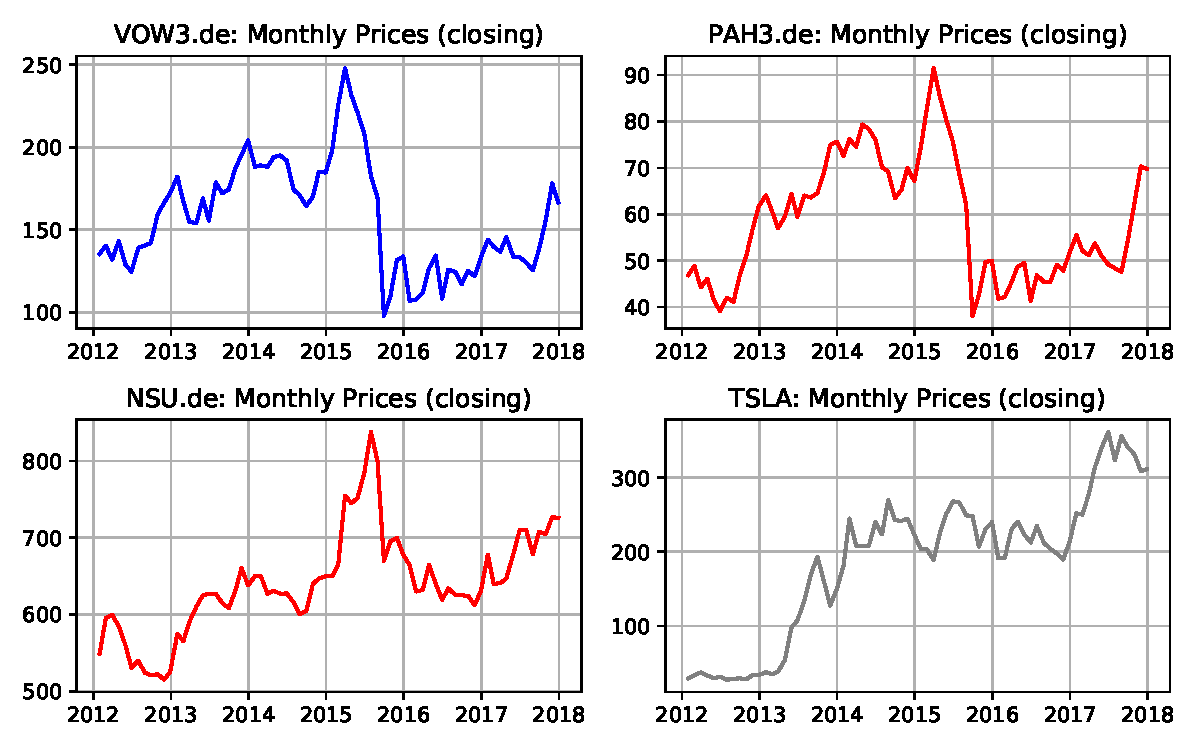
\includegraphics[width=\textwidth]{figures/intro/corr_prices.pdf}
%     \caption{Closing monthly stock prices for four corporations from the automotive industry (clockwise from top left): Volkswagen AG (VOW3.DE), Porsche Automobil Holding SE (PAH3.DE), Tesla, Inc. (TSLA), Audi AG (NSU.DE)}
%     \label{fig:stockprices}
% \end{figure}

% \todo{Find example with american companies}

% The case example for correlating stock prices in Figure~\ref{fig:stockprices} illustrates how the subsidiary corporations Porsche and Audi relate to their parent corporation VW. The huge drop in 2016 represents the emissions scandal which affected all three corporations. Especially the Porsche stock price moves very similar to the stock price of Volkswagen but also the Audi stock price shows some similarity. As an counter example the Tesla stock price is shown which does not reveal any deep relation with the other ones. This first analysis only gives a first insight into the potential relationships between stock corporations. As a part of this thesis I will investigate the dependency of these econometric time series using statistical tests like the Engle–Granger two-step method for testing cointegration between related stock prices.  \todo{Reformulate}